\documentclass[tikz,border=8pt]{standalone}
\usetikzlibrary{arrows.meta}
\begin{document}
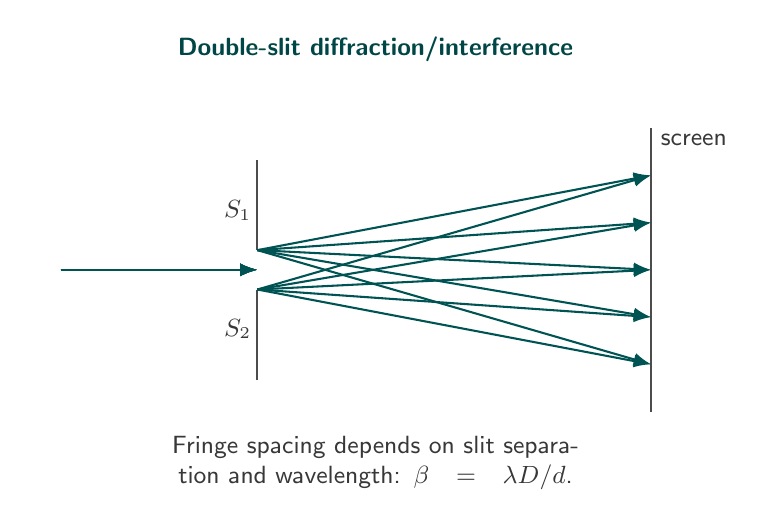
\begin{tikzpicture}[
  ray/.style={-{Latex[length=2.2mm]},draw=teal!65!black,line width=0.75pt},
  line/.style={draw=black!70,line width=0.75pt},
  label/.style={font=\sffamily\small,text=black!78},
  title/.style={font=\sffamily\bfseries\small,text=teal!55!black},
]
\node[title] at (0,2.8) {Double-slit diffraction/interference};
\draw[line] (-1.5,-1.4)--(-1.5,-0.25);
\draw[line] (-1.5,0.25)--(-1.5,1.4);
\node[label] at (-1.75,0.75) {$S_1$};
\node[label] at (-1.75,-0.75) {$S_2$};
\draw[line] (3.5,-1.8)--(3.5,1.8);
\foreach \y in {-1.2,-0.6,0,0.6,1.2}{\draw[ray] (-4,0)--(-1.5,0); \draw[ray] (-1.5,0.25)--(3.5,\y); \draw[ray] (-1.5,-0.25)--(3.5,\y);}
\node[label,right] at (3.5,1.65) {screen};
\node[label,align=center,text width=8.6cm] at (0,-2.45)
  {Fringe spacing depends on slit separation and wavelength: $\beta=\lambda D/d$.};
\end{tikzpicture}
\end{document}
